\input{../head.tex}

\section{Modélisation des filtres passe-haut, passe-bas, et passe-bande}
Dans cette section, nous allons expliquer la méthode que nous avons
utiliseé pour trouver une expression analytique de la tension de sortie 
dans un filtre passe-bas, ainsi que dans un filtre passe-haut. Nous 
étudierons également la combinaison de ces deux filtres: le passe-bande.

Nous avons en réalité utilisé deux méthodes différentes qui, heureusement, 
aboutissent à la même solution. La première méthode utilise ce que nous
avons appris au premier quadrimestre concernant les équations différentielles.
Cette méthode est plus longue et plus compliquée que la deuxième, c'est pourquoi
nous ne la décrirons pas ici.
La deuxième méthode utilise ce que nous avons appris au deuxième quadrimestre 
concernant les équations différentielles et les complexes. 

\subsection{Le filtre passe-bas}
Le filtre passe-bas dans notre haut-parleur a pour but de laisser
passer les basses fréquences et d'atténuer les plus hautes fréquences.

Soit $V_R$ la tension à travers la résistance $R$, $V_C$ la tension à travers
le condensateur $C$, $V_{in}$ la tension d'entrée et $V_{out}$ la tension de
sortie du filtre.

\begin{figure}[!htb]
	\centering
	\begin{circuitikz}
		\draw (0,0) node[ocirc] (A);
		\draw (0,0) to [R=$R$] (2,0);
		\draw (2,0) to [short] (4,0);
		\draw (4,0) node[ocirc] (C);
		\draw (2,0) to [C=$C$] (2,-2);
		\draw (2,-2) to [short] (4,-2);
		\draw (4,-2) node[ocirc] (D);
		\draw (0,-2) to [short] (2,-2);
		\draw (0,-2) node[ocirc] (B);
		\draw (A) to[open, v=$V_ {in}$] (B);
		\draw (C) to[open, v=$V_{out}$] (D);
	\end{circuitikz}
	\caption{Schéma électrique d'un filtre passe-bas}
	\label{lwp_scheme}
\end{figure}

Sur le circuit ci-dessus (Figure \ref{lwp_scheme}), nous pouvons utiliser la loi des tensions de Kirchhoff :

$$V_{in} = V_R + V_{out}$$

Notons $V$ l'amplitude de la tension d'entrée sinusoïdale, et $i(t)$ le courant
en fonction du temps : 

$$V \cdot \cos (\omega t) = R \cdot i(t) + V_C$$

Or, le courant $i(t)$ à travers un condensateur est donné par $C \frac{dV_C}{dt}$, 
l'équation devient alors une équation différentielle en la fonction inconnue $V_C (t)$ :

$$V \cdot \cos (\omega t) = RC\frac{dV_C}{dt}  + V_C$$

Nous pouvons réecrire cette équation de la manière suivante, où $y = V_C(t)$ :

$$RCy' + y = V \cdot \cos (\omega t)$$

Cette équation va être la base de la méthode qui suit. Nous utiliserons également
la condition initiale suivante :

$$y(0) = 0$$

\subsubsection{Résolution de l'équation différentielle}

Nous savons que $\cos (\omega t)$ est égale à la partie réelle de l'exponentielle
complexe $e^{\omega i t}$. Nous réécrivons alors l'équation différentielle de la
manière suivante :

$$RCy' + y = V \cdot e^{\omega i t}$$

Comme pour toute équation différentielle linéaire non-homogène, nous allons travailler
en deux étapes :

\paragraph{Recherche de la solution homogène}

Le polynôme caractéristique de l'équation homogène est :

$$RC \cdot x + 1 = 0$$

Nous obtenons alors $x = \frac{-1}{RC}$ comme racine, et nous trouvons donc comme solution homogène :

$$y_h(t) = A \cdot e^{\frac{-t}{RC}}$$

Où $A$ est une constante appartenant à l'ensemble des réels. % A confirmer, j'ai un doute.

\paragraph{Recherche de la solution particulière}

La solution particulière que nous recherchons est de la forme :

$$y_p(t) = \alpha \cdot e^{\omega i t}$$

Il nous reste donc à déterminer la constante complexe $\alpha$. Pour ce faire,
nous injectons dans l'équation de départ $y_p(t)$ et sa dérivée première. Nous trouvons 
alors :

$$\alpha = \frac{V(1-RC\omega i)}{1+R^2C^2\omega^2}$$

La solution particulière est donc :

$$y_p(t) = \frac{V(1-RC\omega i)}{1+R^2C^2\omega^2} \cdot e^{\omega i t}$$

\paragraph{Solution complète}

La solution finale $y(t)$ est égale à $y_h(t) + y_p(t)$ :

$$y(t) = A \cdot e^{\frac{-t}{RC}} + \frac{V(1-RC\omega i)}{1+R^2C^2\omega^2} \cdot e^{\omega i t}$$

En retransformant ensuite l'exponentielle complexe en sa forme trigonométrique et en ne
gardant que la partie réelle, nous obtenons :

$$y(t) = V_C(t) = \frac{V(\cos (\omega t) + RC\omega \sin (\omega t))}{1 + \omega^2R^2C^2} + A \cdot e^{\frac{-t}{RC}}$$

\paragraph{Élimination de la constante}

Il ne nous reste plus qu'à éliminer la constante $A$ en utilisant la condition initiale.
Nous trouvons enfin :

$$A = -\frac{V}{1 + \omega^2R^2C^2}$$                         

\paragraph{Conclusion}

La tension de sortie en fonction du temps est donc donnée par :

$$V_{out} = \frac{V}{1 + \omega^2R^2C^2} \cdot (\cos (\omega t) + RC\omega \sin (\omega t) - e^{\frac{-t}{RC}})$$

Nous pouvons ensuite réécrire cette formule de manière à faire apparaître
le déphasage de la tension de sortie par rapport à la tension d'entrée. En transformant
$y_p(t)$ en utilisant la notation exponentielle $|z|e^{\phi i}$ d'un couple de la forme 
$a+bi$ et en utilisant ensuite la notation trigonométrique d'une exponentielle complexe,
nous trouvons, après quelques simplifications et mises en évidence :

$$V_{out} = \frac{V}{\sqrt{1 + R^2\omega^2C^2}}
\left(-\frac{e^{\frac{-t}{RC}}}{\sqrt{1 + R^2\omega^2C^2}} + \cos(\arctan(-RC\omega) + \omega t)\right)
$$

Il apparaît donc que le déphasage entre $V_{out}$ et $V_{in}$ est $-\arctan(RC\omega) = -\arctan(2\pi fRC)$.
Ce déphasage augmente donc linéairement avec $\omega$ et est dû au temps que met le condensateur
à se charger. % A vérifier

\subsubsection{Vérification des résultats}

Une première vérification que l'on peut faire est de vérifier que $V_{out}$ tend vers \numprint{0}
lorsque $\omega$ tend vers l'infini. C'est bien le cas ici puisque $\omega^2$ est au dénominateur.

Nous pouvons ensuite regarder les graphes de $V_{out}$, $V_{in}$ (Figure \ref{lwp_voltages}) et $V_{out} / V_{in}$
(Figure \ref{lwp_ratio}). Les résultats sont encourageants.

\begin{figure}[!htb]
	\centering
	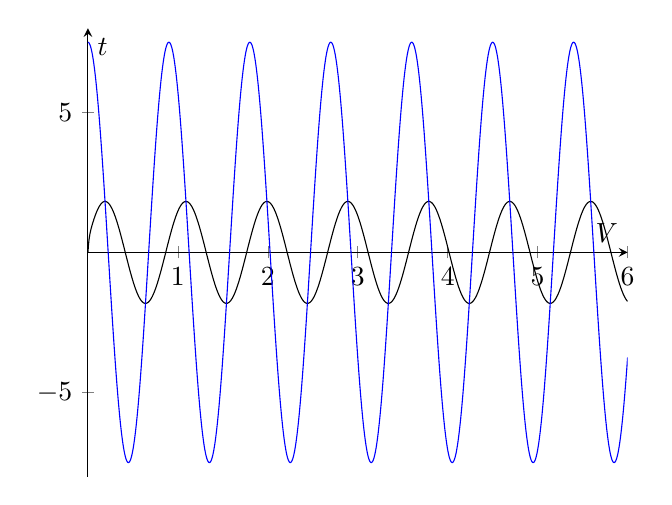
\begin{tikzpicture}[>=stealth]
    \begin{axis}[
        xmin=0,xmax=6,
        ymin=-8,ymax=8,
        axis x line=middle,
        axis y line=middle,
        axis line style=->,
        xlabel={$V$},
        ylabel={$t$},
        ]
				
        \addplot[no marks,black,-] expression[domain=0:6,samples=1000]
						{((7.5)/(sqrt(1 + 1000^2 * 0.00001^2 * 400^2))) * (((-2.718^((-x)/(1000*0.00001)))/(sqrt(1 + 1000^2 * 0.00001^2 * 400^2))) 
						+ cos(atan(-1000*0.00001*400) + 400*x))} 
						node[pos=0.65,anchor=south west]{$$};
						
				\addplot[no marks,blue,-] expression[domain=0:6,samples=1000]
						{7.5 * cos(400 * x)} 
						node[pos=0.65,anchor=south west]{$$}; 

    \end{axis}
	\end{tikzpicture}
	\caption{Graphe de $V_{out}$ (en noir) et $V_{in}$ (en bleu) pour les valeurs suivantes : $V_{max} = \unit{7.5}{\volt}$, $C = \unit{0.00001}{\farad}$,
						$R = \unit{1000}{\ohm}$ et $f = \unit{63.66}{\hertz}$}
	\label{lwp_voltages}
\end{figure}

\begin{figure}[!htb]
	\centering
	\begin{tikzpicture}[>=stealth]
    \begin{axis}[
        xmin=0,xmax=1400,
        ymin=0,ymax=1.2,
        axis x line=middle,
        axis y line=middle,
        axis line style=->,
        xlabel={$f$},
        ylabel={$V_{out} / V_{in}$},
        ]
				
				\addplot[no marks,green,-] expression[domain=0:1400,samples=100]
						% Formule par rapport aux expressions obtenues, un peu décallée
						% {(((7.5)/(sqrt(1 + 100^2 * 0.00001^2 * (2*3.14*x)^2))) * (((-2.718^((-100*0.00001)/(100*0.00001)))/(sqrt(1 + 100^2 * 
						% 0.00001^2 * (2*3.14*x)^2))) + cos(atan(-100*0.00001*2*3.14*x) + 2*3.14*x*100*0.00001)))/(7.5 * cos(2*3.14*x*100*0.00001))}
						{(1 + (2*3.14*x*100*0.00001)^2)^(-0.5)}
						node[pos=0.65,anchor=south west]{$$}; 
    \end{axis}
	\end{tikzpicture}
	\caption{Graphe de $V_{out} / V_{in} = \frac{1}{\sqrt{1 + (RC\omega)^2}}$ pour les valeurs suivantes : $R = \unit{100}{\ohm}$ et $C = {\unit{0.00001}{\farad}}$.}
	\label{lwp_ratio}
\end{figure}

\bigbreak

\subsection{Le filtre passe-haut}
Le filtre passe-haut a le rôle inverse du filtre passe-bas : il atténue les
basses fréquences et laisse passer les hautes fréquences.

Soit $V_R$ la tension à travers la résistance $R$, $V_C$ la tension à travers
le condensateur $C$, $V_{in}$ la tension d'entrée et $V_{out}$ la tension de
sortie du filtre.

\begin{figure}[!htb]
	\centering
	\begin{circuitikz}
		\draw (0,0) node[ocirc] (A);
		\draw (0,0) to [C=$C$] (2,0);
		\draw (2,0) to [short] (4,0);
		\draw (4,0) node[ocirc] (C);
		\draw (2,0) to [R=$R$] (2,-2);
		\draw (2,-2) to [short] (4,-2);
		\draw (4,-2) node[ocirc] (D);
		\draw (0,-2) to [short] (2,-2);
		\draw (0,-2) node[ocirc] (B);
		\draw (A) to[open, v=$V_ {in}$] (B);
		\draw (C) to[open, v=$V_{out}$] (D);
	\end{circuitikz}
	\caption{Schéma électrique d'un filtre passe-haut.}
	\label{hgp_scheme}
\end{figure}

Sur la Figure \ref{hgp_scheme}, la loi des tensions de Kirchhoff donne la même équation que pour le filtre passe-bas :

$$V_{in} = V_R + V_C$$

Cette fois, $V_{out} = V_R$. Or, nous connaissons déjà $V_C$ que nous avons calculé dans
le section précédente. Nous avons alors simplement :

$$V_R = V_{in} - V_C$$

$$V_{out} = \frac{V}{\sqrt{1 + R^2\omega^2C^2}}
\left(\frac{e^{\frac{-t}{RC}}}{\sqrt{1 + R^2\omega^2C^2}} - \cos(\arctan(-RC\omega) + \omega t) \right) + \cos(\omega t)$$

Le déphasage reste donc le même que pour le filtre passe-bas.

\subsubsection{Vérification des résultats}

Pour le filtre passe-haut, nous allons cette fois vérifier que lorsque $\omega$ tend vers \numprint{0}, nous avons
$V_{out}$ qui tend vers \numprint{0} également. Une fois de plus, c'est bien le cas.

Nous pouvons ensuite comparer les graphes de $V_{out}$, $V_{in}$ (Figure \ref{hgp_voltages}) et $V_{out} / V_{in}$
(Figure \ref{hgp_ratio}). Le déphasage apparaît clairement, et les fréquences les plus basses sont effectivement atténuées.

\begin{figure}[!htb]
	\centering
	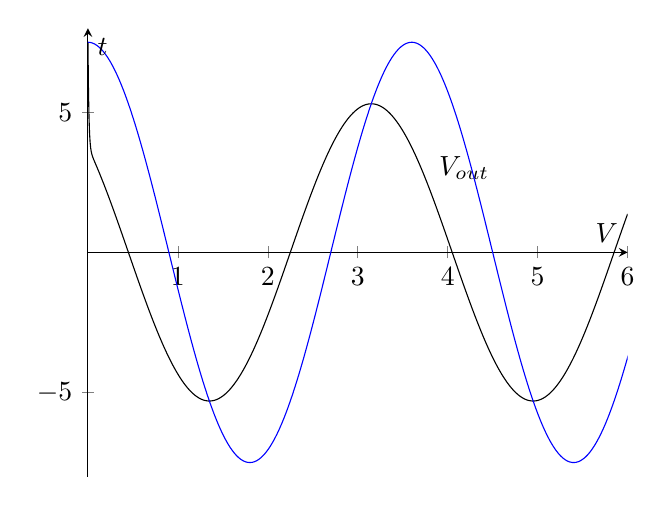
\begin{tikzpicture}[>=stealth]
    \begin{axis}[
        xmin=0,xmax=6,
        ymin=-8,ymax=8,
        axis x line=middle,
        axis y line=middle,
        axis line style=->,
        xlabel={$V$},
        ylabel={$t$},
        ]
				
        \addplot[no marks,black,-] expression[domain=0:6,samples=1000]
						{(7.5 * cos(100*x)) - ((7.5)/(sqrt(1 + 1000^2 * 0.00001^2 * 100^2))) * (((-2.718^((-x)/(1000*0.00001)))/(sqrt(1 + 1000^2 *
						0.00001^2 * 100^2))) + cos(atan(-1000*0.00001*100) + 100*x))} 
						node[pos=0.65,anchor=south west]{$V_{out}$};
						
				\addplot[no marks,blue,-] expression[domain=0:25,samples=1000]
						{7.5 * cos(100 * x)} 
						node[pos=0.65,anchor=south west]{$V_{in}$}; 
				
    \end{axis}
	\end{tikzpicture}
	\caption{Graphe de $V_{out}$ et $V_{in}$ pour les valeurs suivantes : $V_{max} = \unit{7.5}{\volt}$, $C = \unit{0.00001}{\farad}$,
					$R = \unit{1000}{\ohm}$ et $f = \unit{15.91}{\hertz}$}
	\label{hgp_voltages}
\end{figure}

\begin{figure}[!htb]
	\centering
	\begin{tikzpicture}[>=stealth]
    \begin{axis}[
        xmin=0,xmax=1400,
        ymin=0,ymax=1,
        axis x line=middle,
        axis y line=middle,
        axis line style=->,
        xlabel={$f$},
        ylabel={$V_{out}/V_{in}$},
        ]

				\addplot[no marks,green,-] expression[domain=0:1400,samples=100]
				% Formule obtenue avec nos expressions, décallée de 0.4 vers le haut.
				%		{((7.5 * cos(2*3.14*x*100*0.00001)) - ((7.5)/(sqrt(1 + 100^2 * 0.00001^2 * (2*3.14*x)^2))) * 		
				%	(((-2.718^((-100*0.00001)/(100*0.00001)))/(sqrt(1 + 100^2 *0.00001^2 * (2*3.14*x)^2))) + cos(atan(-100*0.00001*2*3.14*x) +
				%	2*3.14*x*100*0.00001)))/(7.5 * cos(2*3.14*x*100*0.00001))}
				{(1 + (1)/((2*3.14*x*100*0.00001)^2))^(-0.5)}
						node[pos=0.65,anchor=south west]{$$}; 

    \end{axis}
	\end{tikzpicture}
	\caption{Graphe de $V_{out} / V_{in} = 1 + \frac{1}{\sqrt{1}{\sqrt{1+(RC\omega)^2}}}$ pour les valeurs suivantes : $R = \unit{100}{\ohm}$ et $C = {\unit{0.0001}{\farad}}$.}
	\label{hgp_ratio}
\end{figure}

\bigbreak

\subsection{Le filtre passe-bande}
Le filtre passe-bande sert, comme son nom l'indique, à laisser passer une certaine
bande de fréquence. Il est constitué d'un filtre passe-haut suivi d'un passe-bas, 
ou inversément. Les fréquences de coupure respectives des filtres déterminent 
l'ampleur de la bande passante. Plus la résistance pour le filtre passe-bas 
(resp.passe-haut) est grande(resp.petite), plus la bande passante est large, 
étant donné que la fréquence de coupure est inversément proportionnelle à la 
résistance. Nous nous intéresserons ici à un signal passant d'abord par un filtre 
passe-haut, et ensuite par le filtre passe-bas.

Soit $V_{in,1}$ la tension à l'entrée du filtre passe-bas, $R_{1}$ la résistance, 
et $C_{1}$ la capacité. Dans la section précédente, nous sommes arrivés au résultat suivant:

$$V_{out,1} = \frac{V_{in,1}}{\sqrt{1 + R_{1}^2\omega^2C_{1}^2}}

(-\frac{e^{\frac{-t}{R_{1}C_{1}}}}{\sqrt{1 + R_{1}^2\omega^2C_{1}^2}} + 
\cos(\arctan(-R_{1}C_{1}\omega) + \omega t))$$

Cette tension de sortie du filtre passe-bas sera notre tension d'entrée pour le 
filtre passe-haut. Précédemment, dans la section concernant le filtre passe-haut,
nous trouvions :

$$V_{out,2} = \frac{V_{in,2}}{\sqrt{1 + R_{2}^2\omega^2C_{2}^2}}
\left(\frac{e^{\frac{-t}{R_{2}C_{2}}}}{\sqrt{1 + R_{2}^2\omega^2C_{2}^2}} - 
\cos(\arctan(-R_{2}C_{2}\omega) + \omega t)\right) + V_{in,}\cos(\omega t)$$

où $V_{in,2}$ est la tension à l'entrée du filtre passe-haut, $R_{2}$ la résistance, 
et $C_{2}$ la capacité. Étant donné que nous disposons d'un adaptateur d'impédance, 
nous pouvons nous permettre d'utiliser ces deux équations obtenues séparément.
En remplaçant $V_{in,2}$ par $V_{out,1}$, la tension à la sortie du passe-bas, nous 
trouvons $V_{out,3}$, la tension de sortie finale.
Après simplifications, nous obtenons:

$$V_{out,3} = \frac{V_{out,1} \cdot V_{out,2}}{V_{in,1}}$$

\begin{figure}[ht!]
\centering
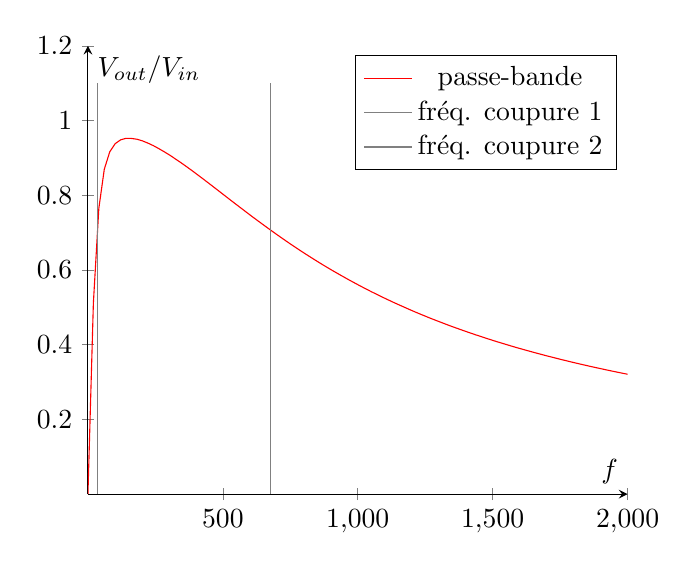
\begin{tikzpicture}[>=stealth]
    \begin{axis}[
        xmin=0,xmax=2000,
        ymin=0,ymax=1.2,
        axis x line=middle,
        axis y line=middle,
        axis line style=->,
        xlabel={$f$},
        ylabel={$V_{out} / V_{in}$},
				legend entries = {passe-bande, fréq. coupure 1, fréq. coupure 2}
        ]

\addplot[no marks,red,-] expression[domain=0:2000,samples=100]
{(((2*3.14*x*10000*0.00000047)*(1 + (2*3.14*x*10000*0.00000047)^2)^(-0.5))*
((1 + (2*3.14*x*500*0.00000047)^2)^(-0.5)))};
\addplot[no marks, gray] coordinates
{(33.86,0) (33.86,1.1)};
\addplot[no marks, gray] coordinates
{(677.26,0) (677.26,1.1)};


\end{axis}
\end{tikzpicture}
\caption{Graphe de $V_{out} / V_{in}$ pour le filtre passe-bande, pour les valeurs suivantes: $R_{1} = \unit{500}{\ohm}$, $R_{2} = \unit{10000}{\ohm}$, et $C = {\unit{0.00000047}{\farad}}$}
\label{lwp_ratio}
\end{figure}
\subsubsection{Vérification des résultats}

Au vu du graphe de $V_{out,3} / V_{in,1}$ de l'équation obtenue pour le passe-bande, nous pouvons
valider notre résultat, étant donné que l'allure du graphique correspond à nos attentes. En effet,
les fréquences de coupure théoriques représentées sur la figure semblent concorder avec les courbes.

\input{../foot.tex}
